\ProvidesFile{ch-introduction.tex}

\chapter{INTRODUCTION}

International interest in cislunar space has increased significantly in the recent decade \cite{nelson2024moon}. Space domain awareness (SDA) will be critical for the future sustainable development of cislunar space. Compared to SDA near Earth, cislunar SDA faces significant challenges due to highly nonlinear cislunar dynamics, extreme distances, and frequent observation gaps. To add to this complexity, active cislunar spacecraft have the ability to maneuver, which in combintation with the chaotic cislunar dynamics further compounds the extreme nonlinearity of the tracking problem. Additionally, low-thrust propulsion has become an increasingly popular choice for spacecraft because of its high specific impulse, allowing for longer mission durations and smaller fuel fractions. Thus, tracking low-thrust maneuvering spacecraft in cislunar space is a problem of interest. 

Significant research effort has been dedicated to the general maneuvering target tracking problem. Bar-Shalom et al. presents several sequential algorithms to account for the discrete nature of maneuvering objects, most notably the interacting multiple model estimator \cite{bar1989tracking} (IMM) and the variable state dimension estimator \cite{bar2007variable} (VSD). Goff et al. implements a combination of these algorithms specifically for tracking low-thrust maneuvering spacecraft in geocentric orbits \cite{goff2015orbit}. Wetterer et al. utilizes an IMM to track impulsively maneuvering spacecraft in cislunar space \cite{wetterer2022cislunar}.

Other research efforts have been dedicated to manage the nonlinearity of the problem. DeMars et al. model the true uncertainty distribution as a mixture of Gaussian distributions, where the number of Gaussian kernels is adaptively increased and decreased in areas of higher and lower nonlinearity, respectively, where nonlinearity is detected via entropy \cite{demars2013entropy}. They then apply this algorithm to accurately model the uncertainty distribution of a spacecraft in geocentric orbit. Vishwjeet and Singla similarly apply a Gaussian mixture-based approach, instead detecting nonlinearity using the Kolmogorov equation error \cite{vishwajet2018adaptive}. 

% \begin{figure}
%     \centering
%     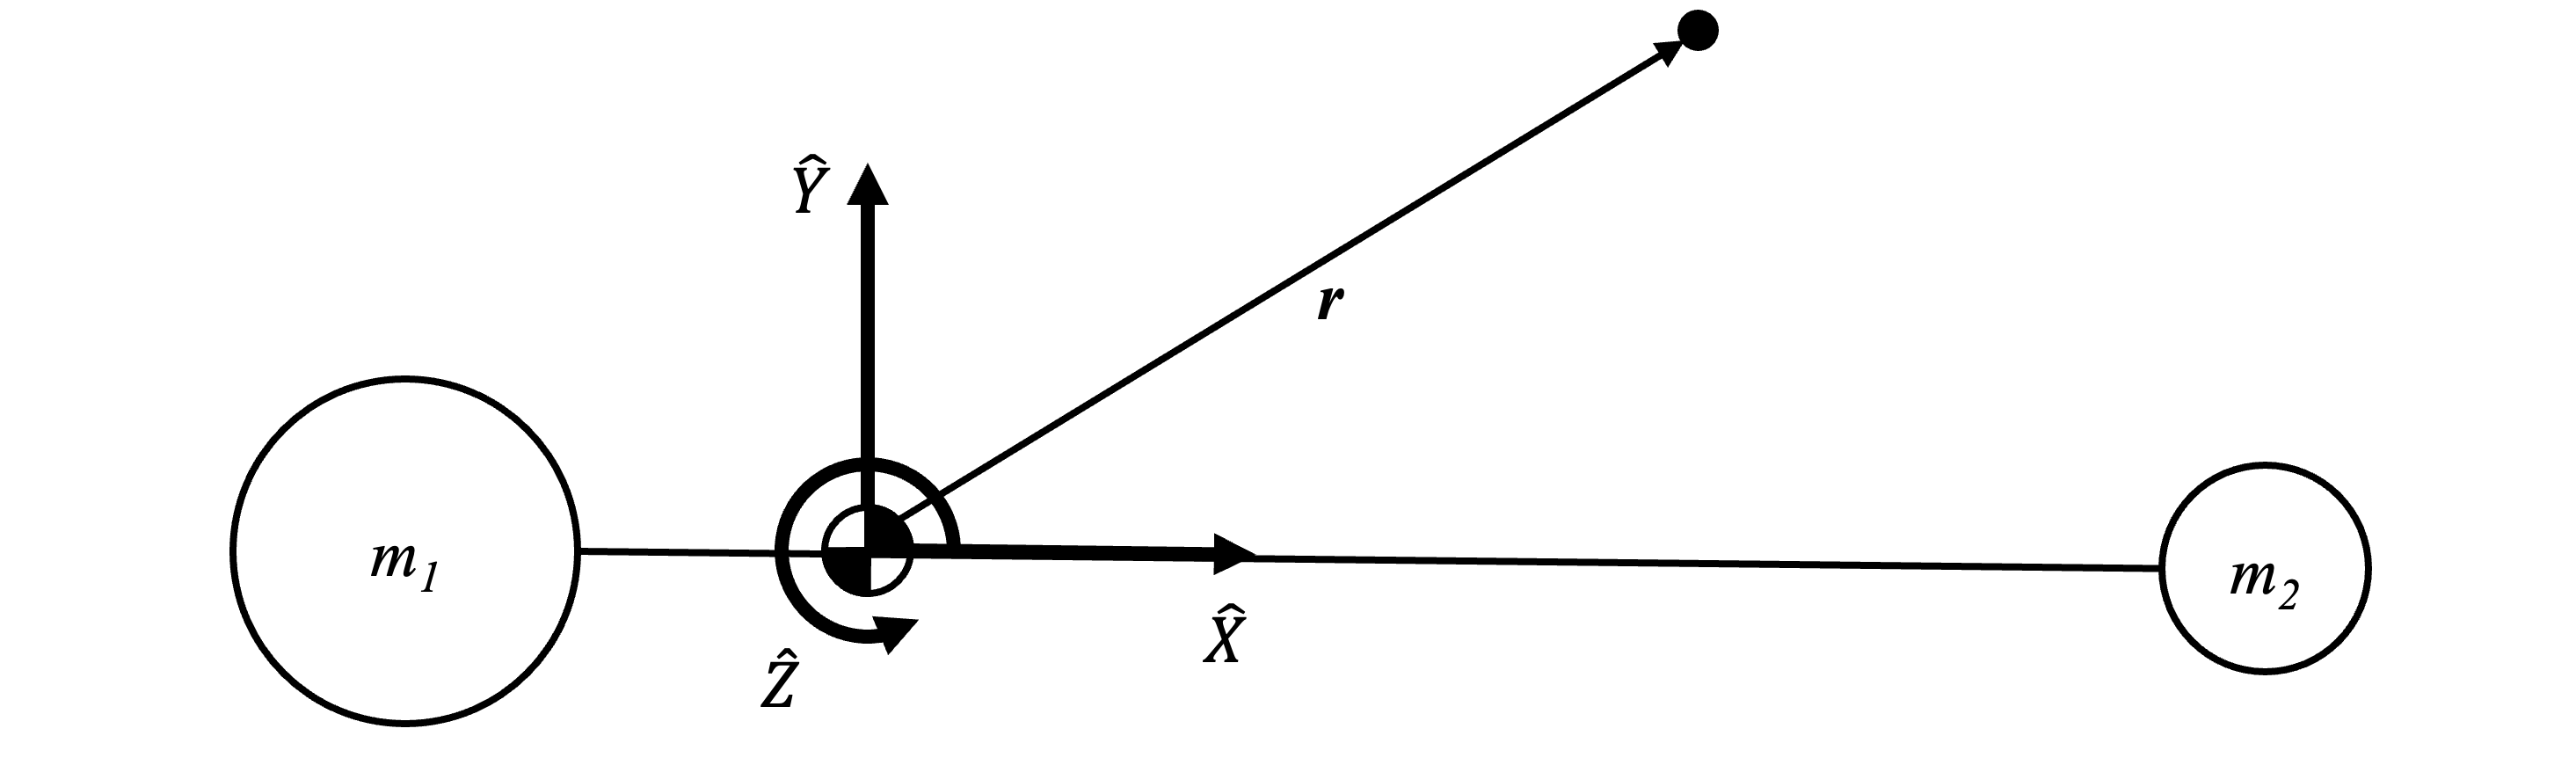
\includegraphics[width=1\linewidth]{Figures/CR3BP.png}
%     \caption{Circular-Restricted Three-Body Problem Coordinate Frame}
%     \label{fig:CR3BP}
% \end{figure}

Iannamorelli and LeGrand combine the adaptive Gaussian mixture and multiple model estimation approaches to simultaneously combat the extreme nonlinearity of cislunar dynamics and account for the maneuvers of a spacecraft \cite{iannamorelli2025adaptive}. Their adaptive Gaussian mixture interacting multiple model estimator (AGMIMM) models maneuvers as zero-mean, Gaussian process noise, so if properly tuned to capture all possible spacecraft maneuvers, the AGMIMM is able to accurately determine where the spacecraft \textit{could} be. However, it is reasonable to assume that the maneuvers of the target spacecraft will be optimal, in which case modeling maneuvers as zero-mean process noise would be overly-conservative. If instead some optimal control law is assumed, given observations of the beginning of a maneuver, it is possible to predict where the spacecraft \textit{should} be at some future time with less uncertainty than by modeling maneuvers as zero-mean process noise. As cislunar SDA becomes more complex with more cislunar spacecraft, decreasing this uncertainty will be critical for correlating tracks of multiple maneuvering targets and allocating limited observational resources.

The concept of using optimal control to improve tracking is explored by Holzinger et al., resulting in the development of the control-distance metric \cite{holzinger2012object}. The control-distance metric characterizes the amount of control effort required to connect two spacecraft states assuming some optimal control, thus allowing the correlation of tracks which are separated by smaller control distances. Lubey and Scheeres apply this framework to develop a sequential estimator, resulting in the Optimal Control-Based Estimator (OCBE) \cite{lubey2013optimal}. The OCBE models any deviation in the state dynamics as an optimal control, which allows both control inputs and mismodeled dynamics to be reconstructed from these deviations. The OCBE is applied by Greaves and Scheeres to the cislunar tracking problem for maneuver detection and reconstruction \cite{greaves2021observation}. These approaches, however, are for the posterior reconstruction and detection of maneuvers rather than for the prior prediction of maneuvers. 

The main contribution of this paper is the implementation of an assumed optimal control policy directly into the dynamics of an adaptive multiple-model estimator. An IMM with two modes is utilized, where the non-maneuvering (coasting) mode assumes ballistic dynamics, and the maneuvering (thrusting) mode assumes a minimum-time optimal control policy. The dynamics of the minimum-time optimal control policy are obtained using Pontryagin's minimum principle \cite{pontryagin1962}. This optimal control IMM (OCIMM) is used to track a cislunar spacecraft performing a low-thrust transfer between two periodic cislunar orbits under a fuel-optimal control policy, whose thrusting arcs follow the same dynamics of a time-optimal policy. The OCIMM is shown to be able to accurately predict the future control inputs of the target spacecraft, even during observation gaps and periods of rapidly changing control. This results in superior estimation performance compared to a traditional IMM. 
